\section{Approach to Software Development}
%%%%%%%%%%%%%%%%%%%%%%%%%%%%%%%%%%%%%%%%%%%%%%%%%
\frame
{
  \Large
  \begin{block}{}
    \center{\bf Sidebar: Important websites}
    \begin{itemize}
      \item \href{http://libmesh.sourceforge.net}{Primary website}
      \item \href{http://github.com/libMesh/libmesh}{Revision Control \& Collaboration with GitHub}
      \item \href{http://buildbot.ices.utexas.edu:8010/waterfall}{Continuous Integration with Buildbot}
        %% \begin{itemize}
        %%   \item \href{http://buildbot.ices.utexas.edu:8010/builders/libmesh\%2Fmaster}{Vanilla Master}
        %%   \item \href{http://buildbot.ices.utexas.edu:8010/builders/libmesh\%2Fmaster%2Bsl6options}{Options}
        %% \end{itemize}
    \end{itemize}
  \end{block}
}


\frame
{
\frametitle{\url{http://libmesh.sourceforge.net}}

\centerline{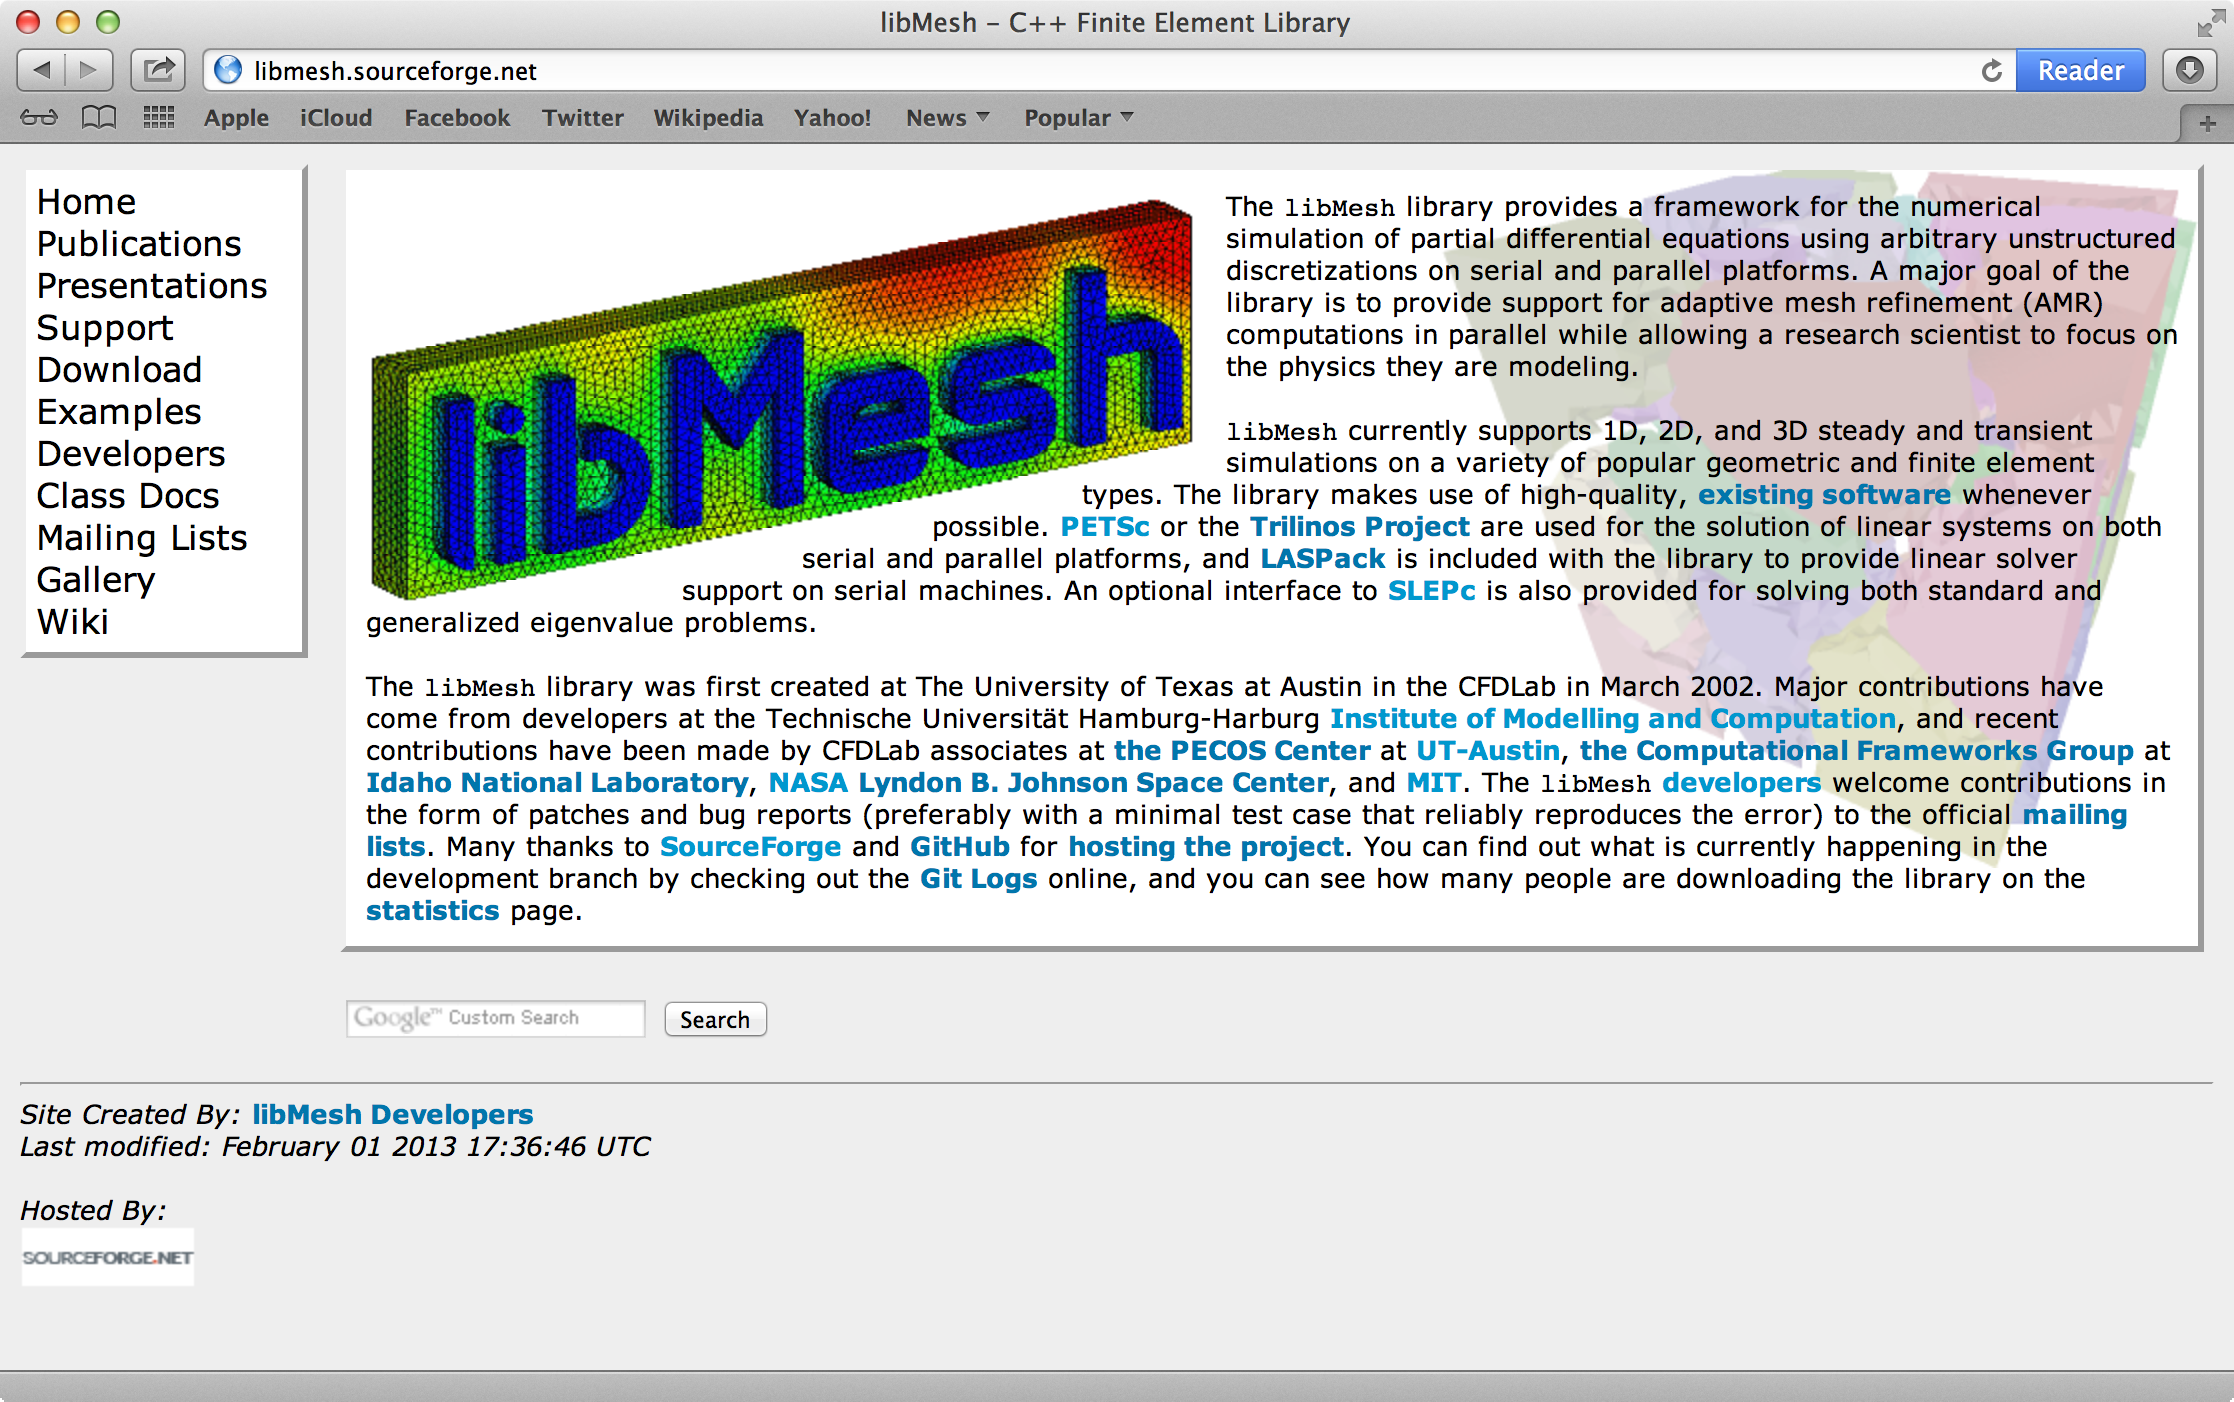
\includegraphics[width=0.85\textwidth]{trivia/libmesh_site}}
}


\frame
{
\frametitle{\url{http://github.com/libMesh/libmesh}}

\centerline{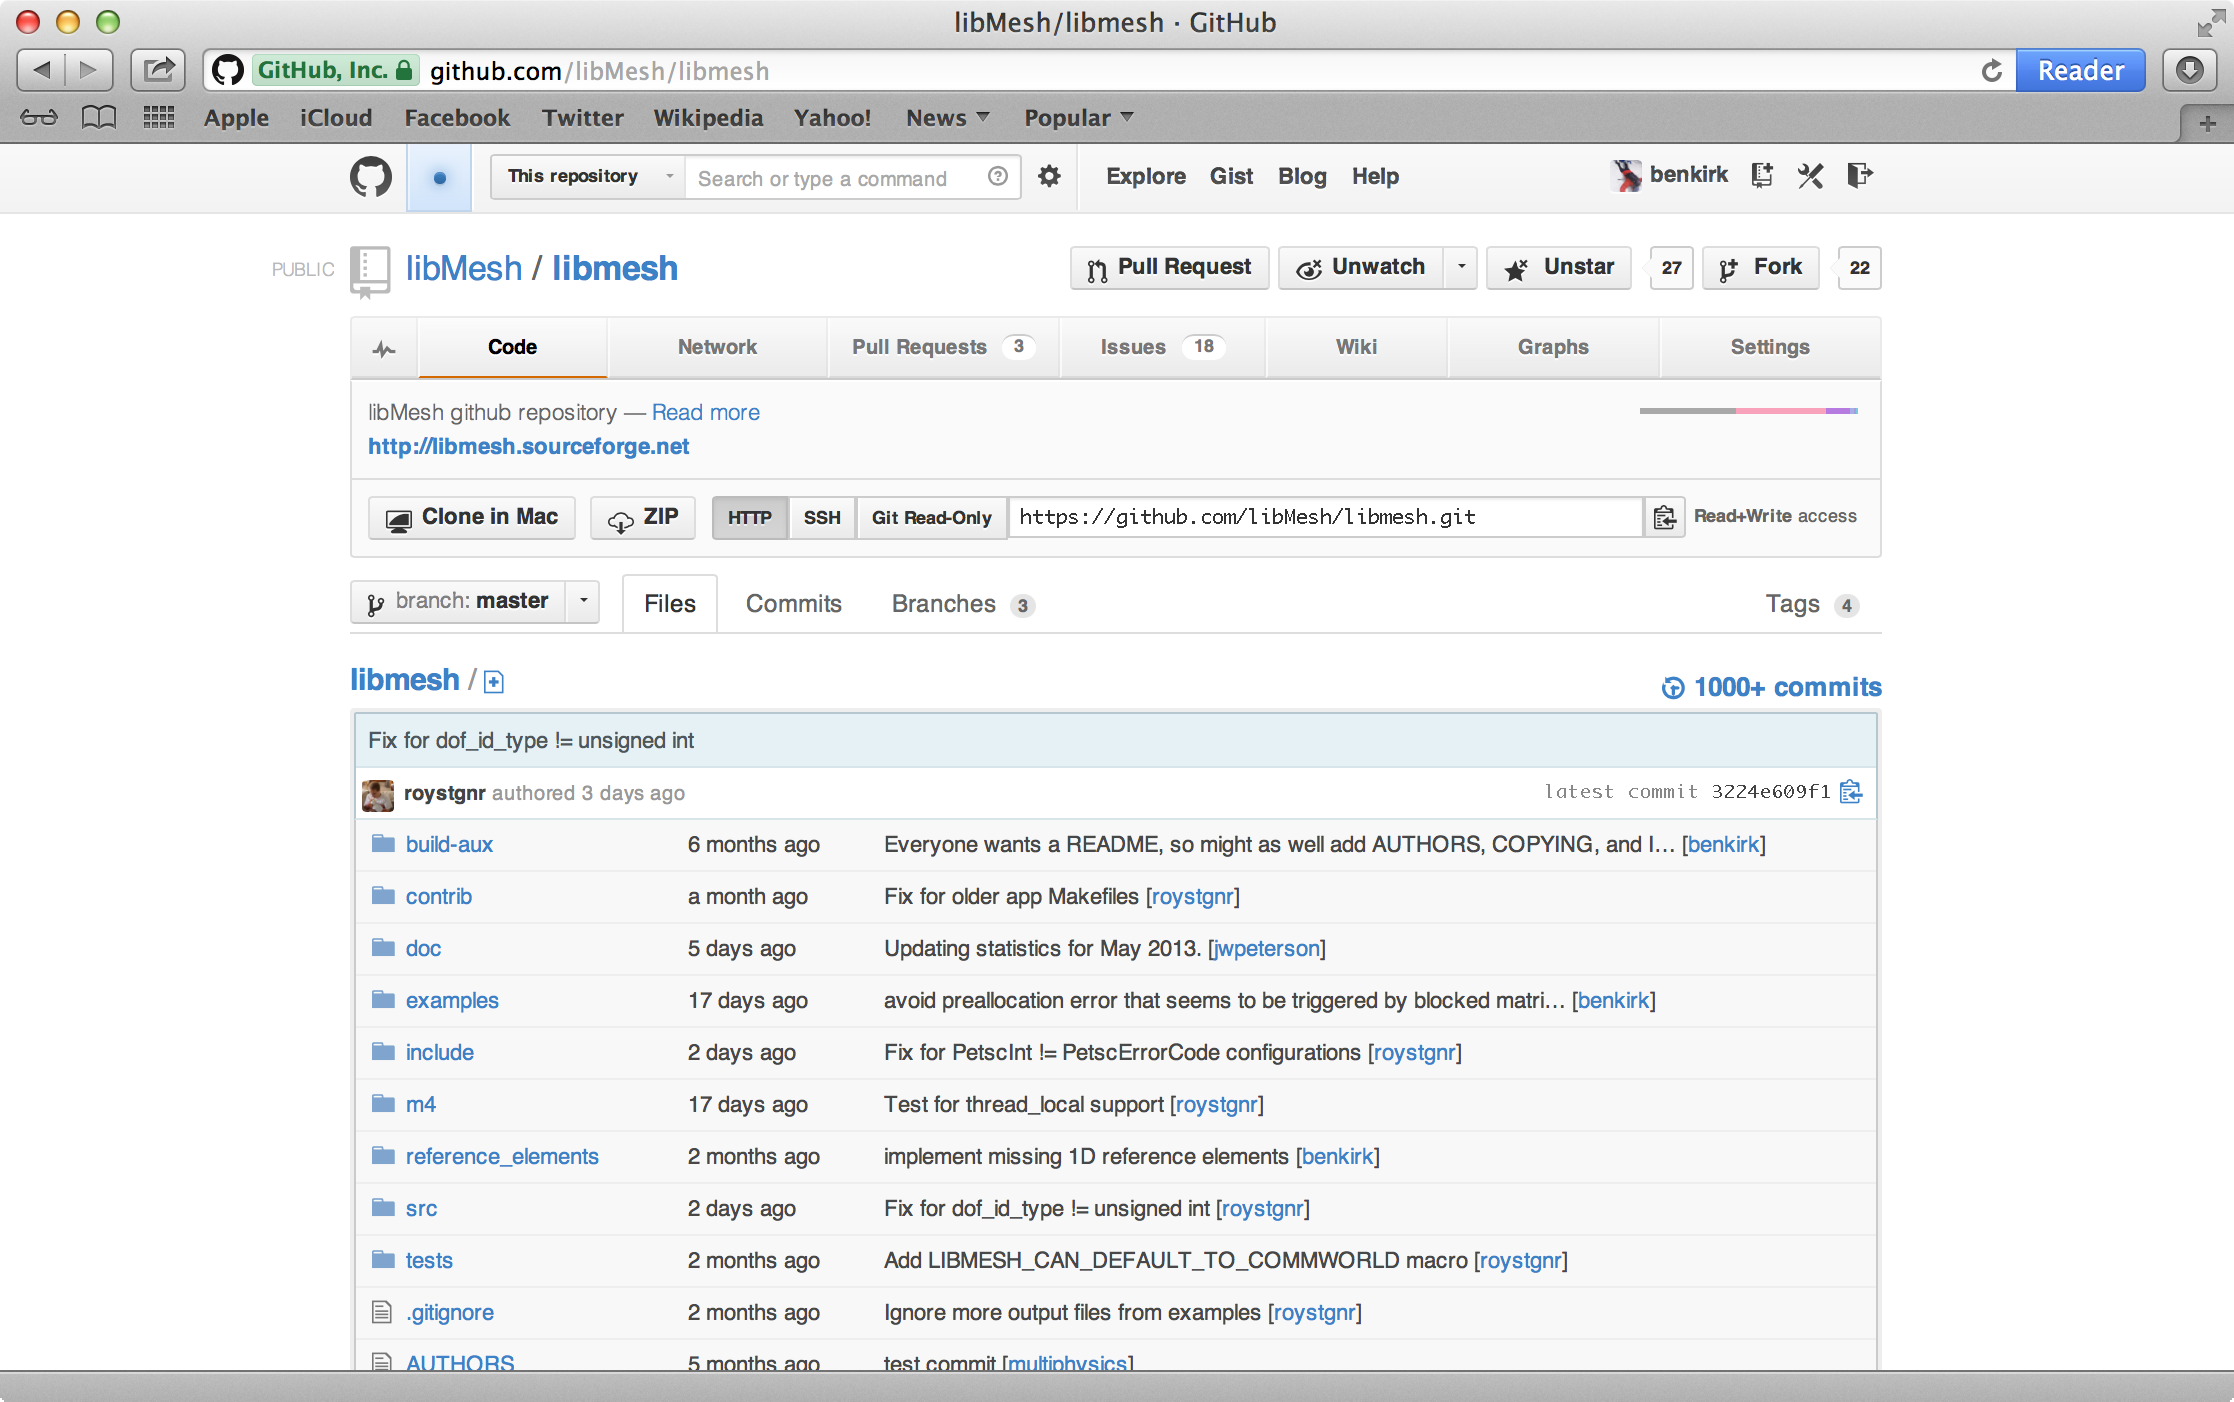
\includegraphics[width=0.85\textwidth]{trivia/github_site}}
}


\frame
{
\frametitle{\scriptsize \url{http://buildbot.ices.utexas.edu:8010/waterfall}}

\centerline{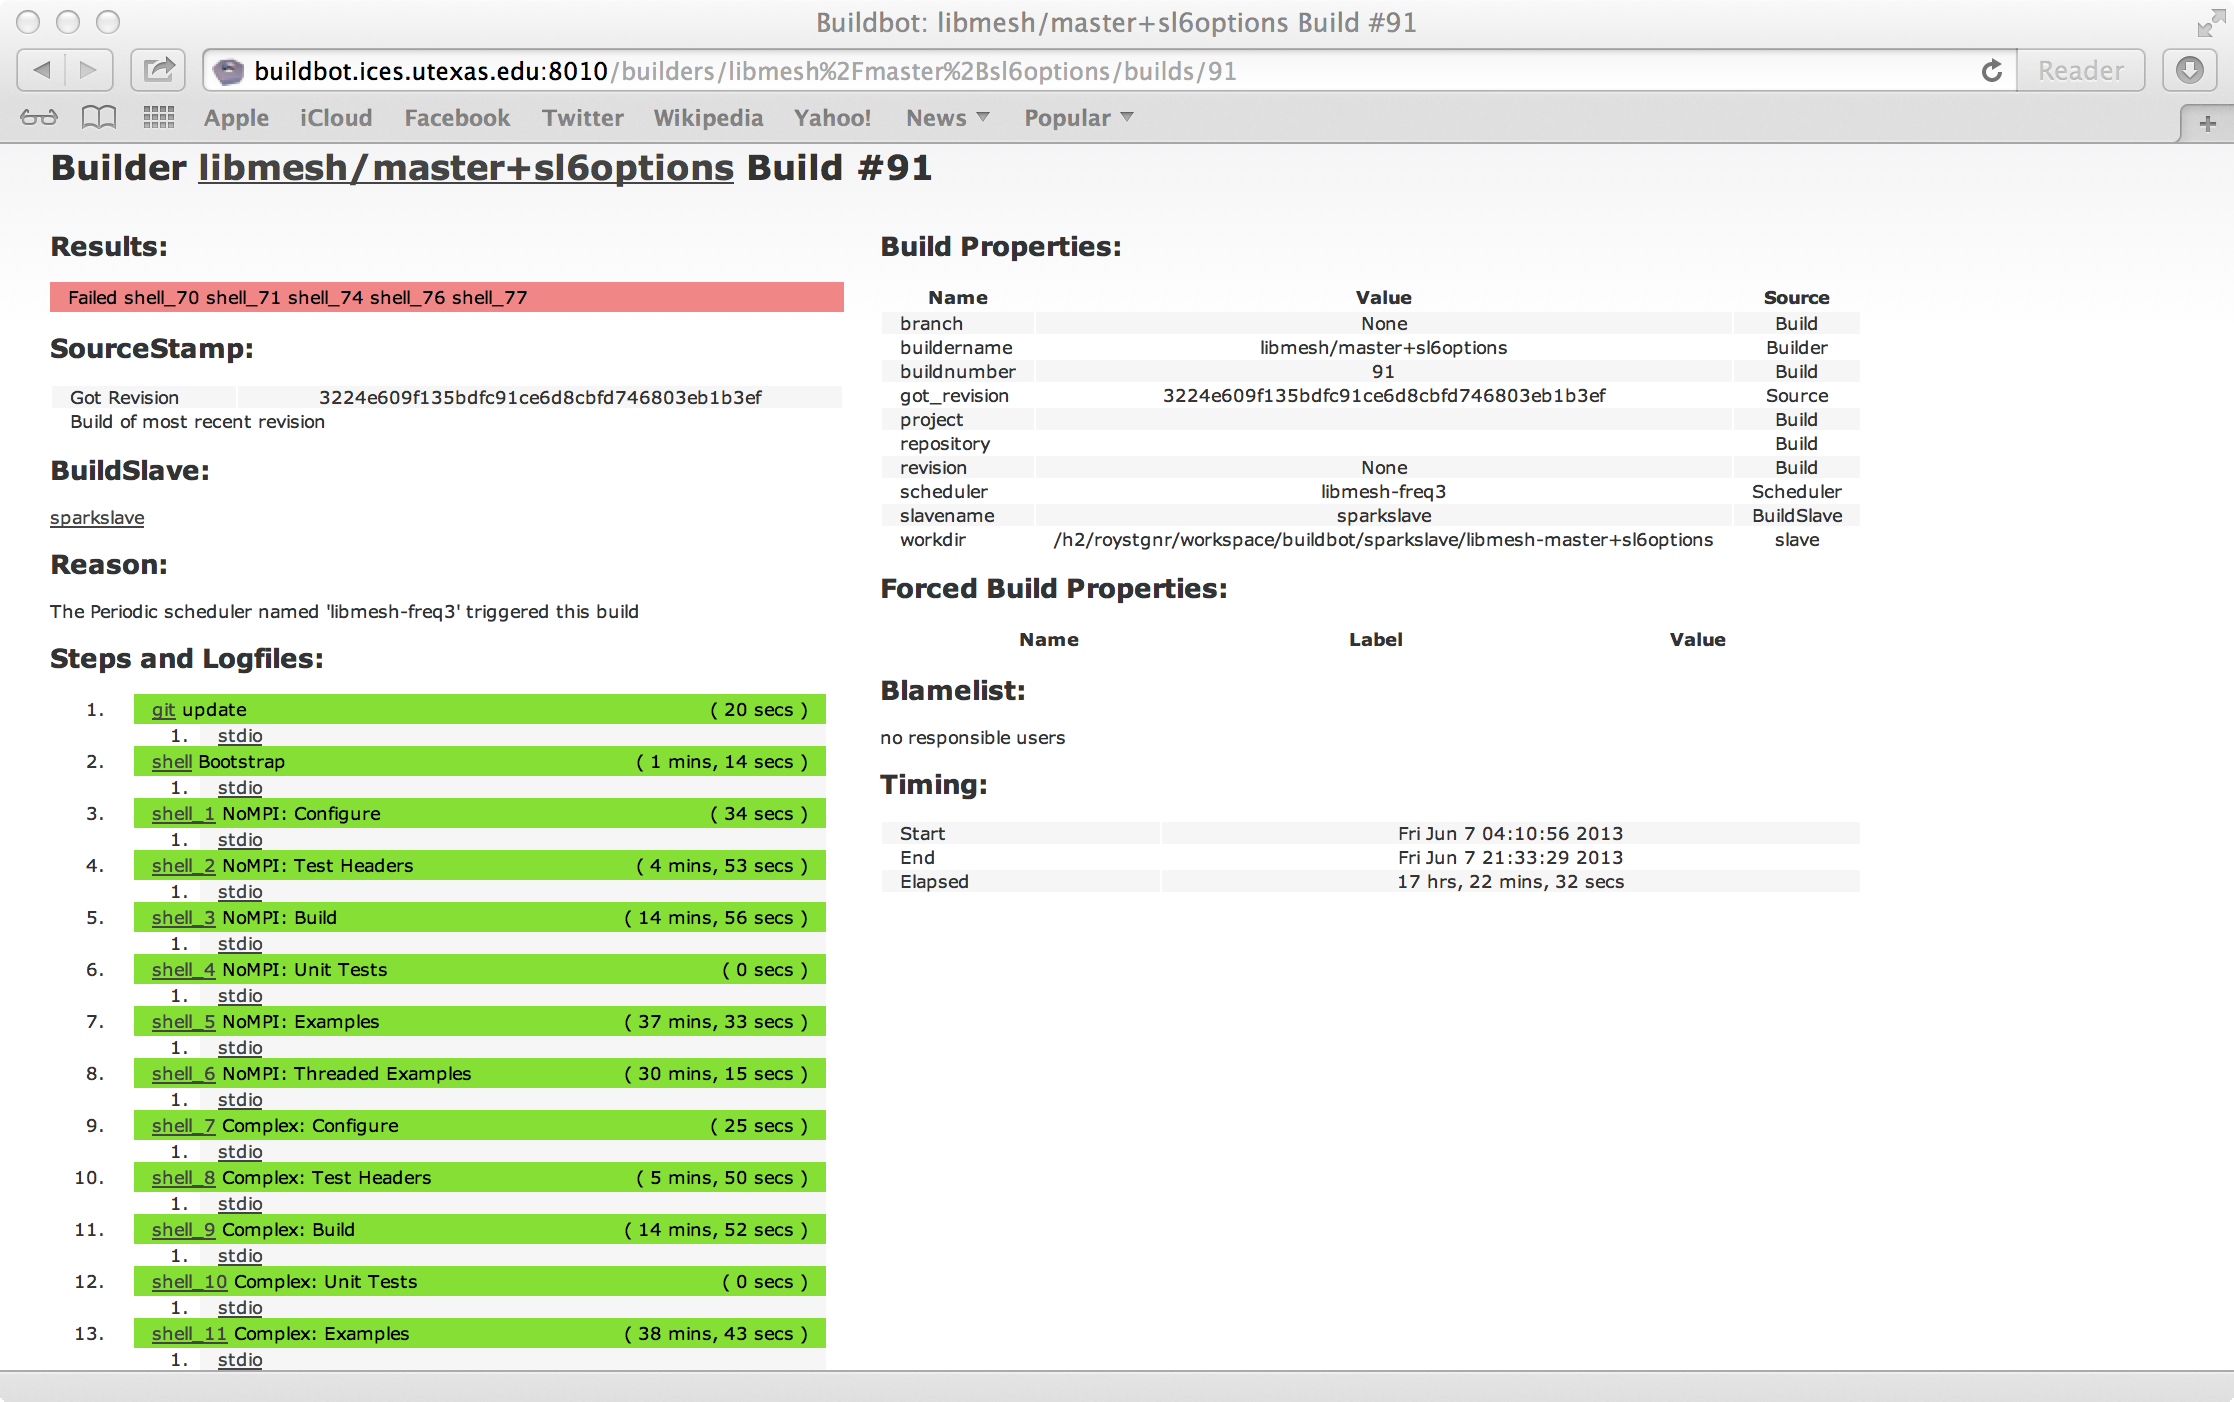
\includegraphics[width=0.85\textwidth]{trivia/buildbot_site}}
}


\begin{frame}[fragile]
  \frametitle{Getting the \libMesh{} Source}

  \begin{block}{}
    \begin{itemize}
    \item \textbf{Blessed, Stable releases:}

      Download prepackaged releases from

      \scriptsize{\url{http://sourceforge.net/projects/libmesh/files/libmesh}}
      \normalsize
    \item \textbf{Development tree:}

      Grab the latest source tree from GitHub:
      \begin{lstlisting}[language=bash]
        git clone git://github.com/libMesh/libmesh.git
      \end{lstlisting}
    \end{itemize}
  \end{block}
\end{frame}


\begin{frame}[fragile]
  \frametitle{Building \libMesh{} from source}

  \begin{block}{Unpack, Configure, Build, Install, \& Test}
    \begin{lstlisting}[language=bash]
      tar jxf libmesh-0.9.1.tar.bz2 && cd libmesh-0.9.1
      ./configure --prefix=`pwd`/install
      make -j 4 && make -j 4 install && make -j 4 check METHODS=opt
      make -j 4 installcheck
    \end{lstlisting}
\end{block}
\end{frame}
